%% Intro
The goal of this section is to develop an analytical queuing model for each component of the system and for the system as a whole. We derive the performance characteristics that the model predicts and compare them with the results obtained in the experiments. We start with a naive model and progressively improve it to better fit our system. 

\subsection{M/M/1}
%% Explain model
In this subsection we build an M/M/1 model based on Section \ref{section:TpForWrites} (Throughput for Writes). 
First of all, we need to define the model boundaries: We choose the net-threads to be the entry point of the system, and the worker threads sending back a response to the clients mark the endpoint of the system. 
The single service of the M/M/1 model represents all the worker threads of the two middlewares together. Note that the service time also includes the memcached RTT because a service having finished serving a job corresponds in the real system to the event of a worker thread sending back a response to the client. The queue in front of the service represents the internal request queues of both middlewares together. 
This is a naive model and has several differences to the actual system which are discussed at the end of this subsection. \\

%% Input parameters of model
\textbf{Input parameters of the model:} %//
\begin{itemize}
\item[--] \textit{mean service rate }$\mu$: We are going to analyze each worker configuration separately. That's why for each worker configuration we choose the maximum observed throughput as an approximation of its mean service rate.
\item[--] \textit{mean arrival rate} $\lambda$: The mean arrival rate is computed as the throughput of the middleware for a specific client load and the analyzed worker configuration. Note that this can only be done because we are in a closed system. For the client load we choose 144 clients because we expect to observe an interesting change in behavior.
\end{itemize}

%% Make predictions based on model and input values
\textbf{Predictions based on the model and the input values:} First we list the metrics we want to predict and also the corresponding formulas. The formulas are derived from operational laws and can be seen in chapter 31 of the book "The Art of Computer Systems Performance Analysis" by Raj Jain\footnote{Raj Jain, The Art of Computer Systems Performance Analysis: Techniques for Experimental Design, Measurement, Simulation, and Modeling, April 1991, ISBN: 978-0471503361.}. We already include the formulas for the M/M/m model of the next subsection. Note that $\varrho$ is the probability of \textit{m} or more jobs in system: \\ $\varrho=[(mp)^m/(m!(1-p))]*p_0$ where $p_0$ is the probability of zero jobs in the system.
\begin{table}[H]
		\centering
	\begin{tabular}{|c|c|c|}
		\hline
		\multicolumn{1}{|c|}{Metric} & \multicolumn{1}{c|}{M/M/1} & \multicolumn{1}{c|}{M/M/m}\\ \hline
		Traffic load/Utilization $\rho$ & $\lambda/\mu$ & $\lambda/(m\mu)$ \\ \hline
		Mean num jobs in queue $E[n_q]$     & $ \rho^{2}/(1 - \rho)$& $\rho \varrho / (1 - \rho)$ \\ \hline
		Mean num jobs in service $E[n_s]$   & $\rho$ & $m \rho$\\ \hline
		Mean num jobs in system $E[n]$      & $\rho / (1-\rho)$ & $m\rho + \rho \varrho / (1 - \rho)$ \\ \hline
		Mean waiting time $E[w]$            & $\rho \frac{1/\mu}{(1 - \rho)}$ & $\varrho/ [m\mu(1 - \rho)]$\\ \hline
		Mean service time $E[s]$            & $1/\mu$ & $1/\mu$ \\ \hline
		Mean response time $E[r]$           & $ (1/\mu)/(1 - \rho)$ & $\frac{1}{\mu} (1 + \frac{\varrho}{m(1 - \rho)})$ \\ \hline
	\end{tabular}
	\label{}
\end{table}

%%Explain
Results are displayed in Table \ref{table:MM1}. 
First note that the traffic intensities $\rho$ are strictly smaller than $1$, thus the stability condition holds.
Utilization for 8, 16 and 32 workers is almost at 100\%, which matches the behaviour of the system in Section \ref{section:TpForWrites} because workers are the bottleneck and the system is fully saturated at 144 client load (see Figure \ref{full_write_tp}).
For 64 workers, the client load of 144 does not reach saturation yet because there are enough workers that process requests. The model correctly predicts the utilization decrease for 64 workers. 

The queue lengths are not accurately predicted, which might be because of the following reasons:
\begin{enumerate}
\item We have a fixed number of requests in the actual system because it is closed but in the model the queue length can increase even further because it corresponds to an open system. The model is not closed because it has a fixed arrival rate and there are no clients that wait for a response.
\item The actual system has two internal request queues instead of one queue.
\item Small changes in utilization around 100\% result in large changes in the queue length because we only have one very fast service. Reaching high utilization of a single fast service has a more negative impact on the queue length than if multiple slower services reach their limit. This implies that for lower utilization we should have more accurate predictions, which is indeed the case, as can be seen from the queue length and the queue waiting time for 64 workers. 
\end{enumerate}
The number of jobs in service is very under-estimated because the model has only one service which cannot process more than one job at a time and thus $E[n_s] \leq 1$. But in the actual system multiple workers can process jobs in parallel and thus we can have more than one job receiving service. This also leads to the number of jobs in system being under-estimated. \\
Total response times are not accurately predicted because the service time is very underestimated and the waiting time is also not accurate because of the same reason the queue length is not accurately predicted. 

\begin{table}[!ht]
	\begin{adjustbox}{center}
		\begin{tabulary}{\linewidth}{ C | C | C | C | c | C | C | C | C | }
			\cline{2-9}	&	\multicolumn{2}{| c |}{\textbf{8 workers}}	&	\multicolumn{2}{| c |}{\textbf{16 workers}}	&	\multicolumn{2}{| c |}{\textbf{32 workers}}	&	\multicolumn{2}{| c |}{\textbf{64 workers}}	\\
			\cline{2-9} &	predicted	&	measured	&	predicted	&	measured	&	predicted	&	measured	&	predicted	&	measured	\\
			\hline	\multicolumn{1}{| c |}{$\mu$ [req/s]}	    &-      &9'249.94&-	&10'891.57	&-	&13'258.34	&-	&15'670.26	\\
			\hline	\multicolumn{1}{| c |}{$\lambda$ [req/s]}	&-      &9'025.93&-	&10'716.8	&-	&13'023.1	&-	&14'519.22	\\
			\hline	\multicolumn{1}{| c |}{$\rho$}	            &0.9758	&-	    &0.984	&-	&0.9823	&-	&0.9265	&-	\\
			\hline	\multicolumn{1}{| c |}{$\mathbb{E}[n_q]$}	&39.32	&59.7	&60.33	&48.39	&54.38	&27.2	&11.69	&6.94	\\
			\hline	\multicolumn{1}{| c |}{$\mathbb{E}[n_s]$}	&0.98	&16	&0.98	&32	&0.98	&64	&0.93	&128	\\
			\hline	\multicolumn{1}{| c |}{$\mathbb{E}[n]$}	    &40.29	&75.7	&61.32	&80.39	&55.36	&91.2	&12.61	&134.94	\\
			\hline	\multicolumn{1}{| c |}{$\mathbb{E}[w]$ [ms]}&4.36	&13.6	&5.63	&9.78	&4.18	&5.12	&0.8	&0.84	\\
			\hline	\multicolumn{1}{| c |}{$\mathbb{E}[s]$ [ms]}&0.11	&1.77	&0.09	&2.99	&0.08	&4.91	&0.06	&7.19	\\
			\hline	\multicolumn{1}{| c |}{$\mathbb{E}[r]$ [ms]}&4.46	&15.37	&5.72	&12.77	&4.25	&10.03	&0.87	&8.03	\\
			\hline
		\end{tabulary}
	\end{adjustbox}	
	\caption{Predicted and measured metrics of the M/M/1 model for all worker configurations under the load of 144 clients.}
	\label{table:MM1}
\end{table}

%% Describe difference between model and actual system
To conclude, we can say that the model is too simple and cannot predict the experiment results very well because of the following differences to the actual system: In reality we have two internal request queues and not only one because we have two middlewares. The worker threads correspond to multiple services that run in parallel and not to a single sequential service. The model represents an open system because jobs arrive at a fixed arrival rate, and there is no flow of requests where finished jobs are again enqueued at the beginning. But the actual system is a closed one. Another difference is that memcached servers and workers are both in the same service instead of considered independently from each other. 

\subsection{M/M/m}
%% Explain model
In this subsection we build an M/M/m model based on Section \ref{section:TpForWrites}. The model consists of multiple services that process and dequeue jobs from a single queue in parallel. A service corresponds to a single worker thread and again the service time includes the memcached RTT. The queue in front of the services represents the internal request queues of both middlewares together like in the M/M/1 model. This is a more accurate model of our system than the M/M/1 model and should lead to better predictions. \\

%% Input parameters of model
\textbf{Input parameters of the model:} 
\begin{itemize}
\item[--] \textit{mean service rate} $\mu$: There are multiple ways to approximate the mean service rate. Either we take the inverse of the shortest observed service time where the service time consists of the worker preprocessing time, the memcached RTT and the worker postprocessing time. Or we take the maximum observed throughput and divide it by the number of services m. We have chosen the second approach because it lead to better predictions.
\item[--] \textit{mean arrival rate} $\lambda$: Average throughput of the middleware like in the M/M/1 model.
\item[--] \textit{number of services} $m$: We have as many services as total number of workers in the system i.e. m = worker configuration x 2.
\end{itemize}

\begin{table}[!ht]
	\begin{adjustbox}{center}
		\begin{tabulary}{\linewidth}{ C | C | C | C | c | C | C | C | C | }
			\cline{2-9}	&	\multicolumn{2}{| c |}{\textbf{8 workers}}	&	\multicolumn{2}{| c |}{\textbf{16 workers}}	&	\multicolumn{2}{| c |}{\textbf{32 workers}}	&	\multicolumn{2}{| c |}{\textbf{64 workers}}	\\
			\cline{2-9} &	predicted	&	measured	&	predicted	&	measured	&	predicted	&	measured	&	predicted	&	measured	\\
			\hline	\multicolumn{1}{| c |}{$\mu$ [req/s]}	    &-      &578.12&-	&340.36	&-	&207.16	&-	&122.42	\\
			\hline	\multicolumn{1}{| c |}{$\lambda$ [req/s]}	&-      &9'025.93&-	&10'716.8	&-	&13'023.1	&-	&14'519.22	\\
			\hline	\multicolumn{1}{| c |}{$\rho$}	            &0.9758	&-	    &0.984	&-	&0.9823	&-	&0.9265	&-	\\
			\hline	\multicolumn{1}{| c |}{$\mathbb{E}[n_q]$}	&35.85	&59.7	&54.87	&48.39	&46.35	&27.2	&3.73	&6.94	\\
			\hline	\multicolumn{1}{| c |}{$\mathbb{E}[n_s]$}	&15.61	&16	&31.49	&32	&62.86	&64	&118.6	&128	\\
			\hline	\multicolumn{1}{| c |}{$\mathbb{E}[n]$}	    &51.46	&75.7	&86.36	&80.39	&109.21	&91.2	&122.33	&134.94	\\
			\hline	\multicolumn{1}{| c |}{$\mathbb{E}[w]$ [ms]}&3.97	&13.6	&5.12	&9.78	&3.56	&5.12	&0.26	&0.84	\\
			\hline	\multicolumn{1}{| c |}{$\mathbb{E}[s]$ [ms]}&1.73	&1.77	&2.94	&2.99	&4.83	&4.91	&8.17	&7.19	\\
			\hline	\multicolumn{1}{| c |}{$\mathbb{E}[r]$ [ms]}&5.7	&15.37	&8.06	&12.77	&8.39	&10.03	&8.43	&8.03	\\
			\hline
		\end{tabulary}
	\end{adjustbox}	
	\caption{Predicted and measured metrics of the M/M/m model for all worker configurations under the load of 144 clients.}
	\label{table:MMm}
\end{table}

%% Make predictions based on model and input values
\textbf{Predictions based on model and input values:} 
Results are displayed in Table \ref{table:MMm}.
First note that the traffic intensities $\rho$ are strictly smaller than $1$, thus the stability condition holds.
The utilization predictions do match the reality pretty good as in the M/M/1 case. We now have higher service times, respectively lower service rates because we consider m services instead of a single one that models all the worker threads together. That's why the service time is now predicted more accurately than in the M/M/1 model where the service time was very short because of the extremely fast service, which lead to underestimated response times. 
Also the number of jobs in the service is predicted more accurately because it has no upper bound of 1 job anymore and thus also the total number of jobs is predicted more accurately. 
Note that still the response times are mostly predicted too optimistic since this is a more ideal model than our system because of the following: 
\begin{enumerate}
    \item If there are jobs in the queue and there are available workers, jobs will be dequeued and processed. But in our system this may not be the case, because a worker may be ready to dequeue but his queue is empty while the queue in the other middleware is not.
    \item Services operate at a fixed ideal service rate, which in a real system may vary. Also an open system has a fixed arrival rate which can be considered more ideal than a closed system that always has to wait for jobs to finish because if a job of a client is processed very slowly, the client cannot send another job during the processing time.
\end{enumerate}
To conclude, we can say that the M/M/m model is more accurate than the M/M/1 model but the predictions are still not perfect because of the mentioned differences to the real system. In both models the whole system is modeled as a black box. To be able to more accurately predict the behavior of the system, we need to model each component of the system which is done in the next subsection. 

%the following differences to the real system remain: The model still only has one queue instead of two separate queues for each middleware. The model represents an open system instead of a closed one. And finally we have queuing model for the system as a whole where the system

\subsection{Network of Queues}

In this subsection we build a network of queues based on Section \ref{section:BaselineWithMW} (Baseline with Middleware). This is an even more accurate model of our system and should lead to better predictions than the M/M/m model.
We consider both the one and two middleware configuration and analyze both read-only and write-only workloads. The number of worker threads is set to a constant. 

\subsubsection{System with one middleware}
%% Explain model
The model is shown in Figure \ref{NoQ_one_mw}. 
It is a closed queuing network, where jobs keep circulating from one queue to the next, i.e. we have a fixed number of jobs which we set equal to the number of clients. 
The network is modeled as a delay center. Delay centers have no queuing and the service time is independent of the load. The network delays can be computed from the measured ping times. \\
The memtier clients are modeled as a delay center because their queuing time is negligible and we adjust their service time to handle numerical instabilities. We only need a single delay center because the network delay between the clients and the middleware is roughly the same for all clients. \\
The net-thread is simulated with an M/M/1 model. It consists of one service because we have one net-thread and the queue represents the Java Selector in front of the net-thread which enqueues arriving requests from the clients. The service time is computed from the difference of timestamps when the net-thread reads a request and when it enqueues it. \\
The workers and the internal request queue is simulated with an M/M/m model where m is the number of workers. The service time includes the worker preprocessing time, the memcached RTT and the worker postprocessing time. We include the memcached servers in this component because of the Single-Resource Possession condition by Denning and Buzen (1978)\footnote{The Art of Computer Systems Performance Analysis by Raj Jain (chapter 32.2).} which states that a job may not be present at two or more devices at the same time.  If memcached servers were modeled as another component, then as soon as a worker sends a job to a memcached server it would take another job from its queue instead of waiting for the response of the memcached server. This would not model the behavior of our system. 

The model is implemented using the \textit{Octave} programming language and the \textit{queuing} package\footnote{Version 1.2.6 downloaded on \url{https://www.moreno.marzolla.name/software/queueing/}}.
Since we use load-dependent service centers (for the workers), we cannot use the basic MVA algorithm because they cannot be modeled using operational laws\footnote{Exercise session slides on network of queues (page 20).}. In this case we have to use the extended MVA algorithm, which is implemented in the mentioned queuing package of Octave.

\begin{figure}[!ht]
    \centering
	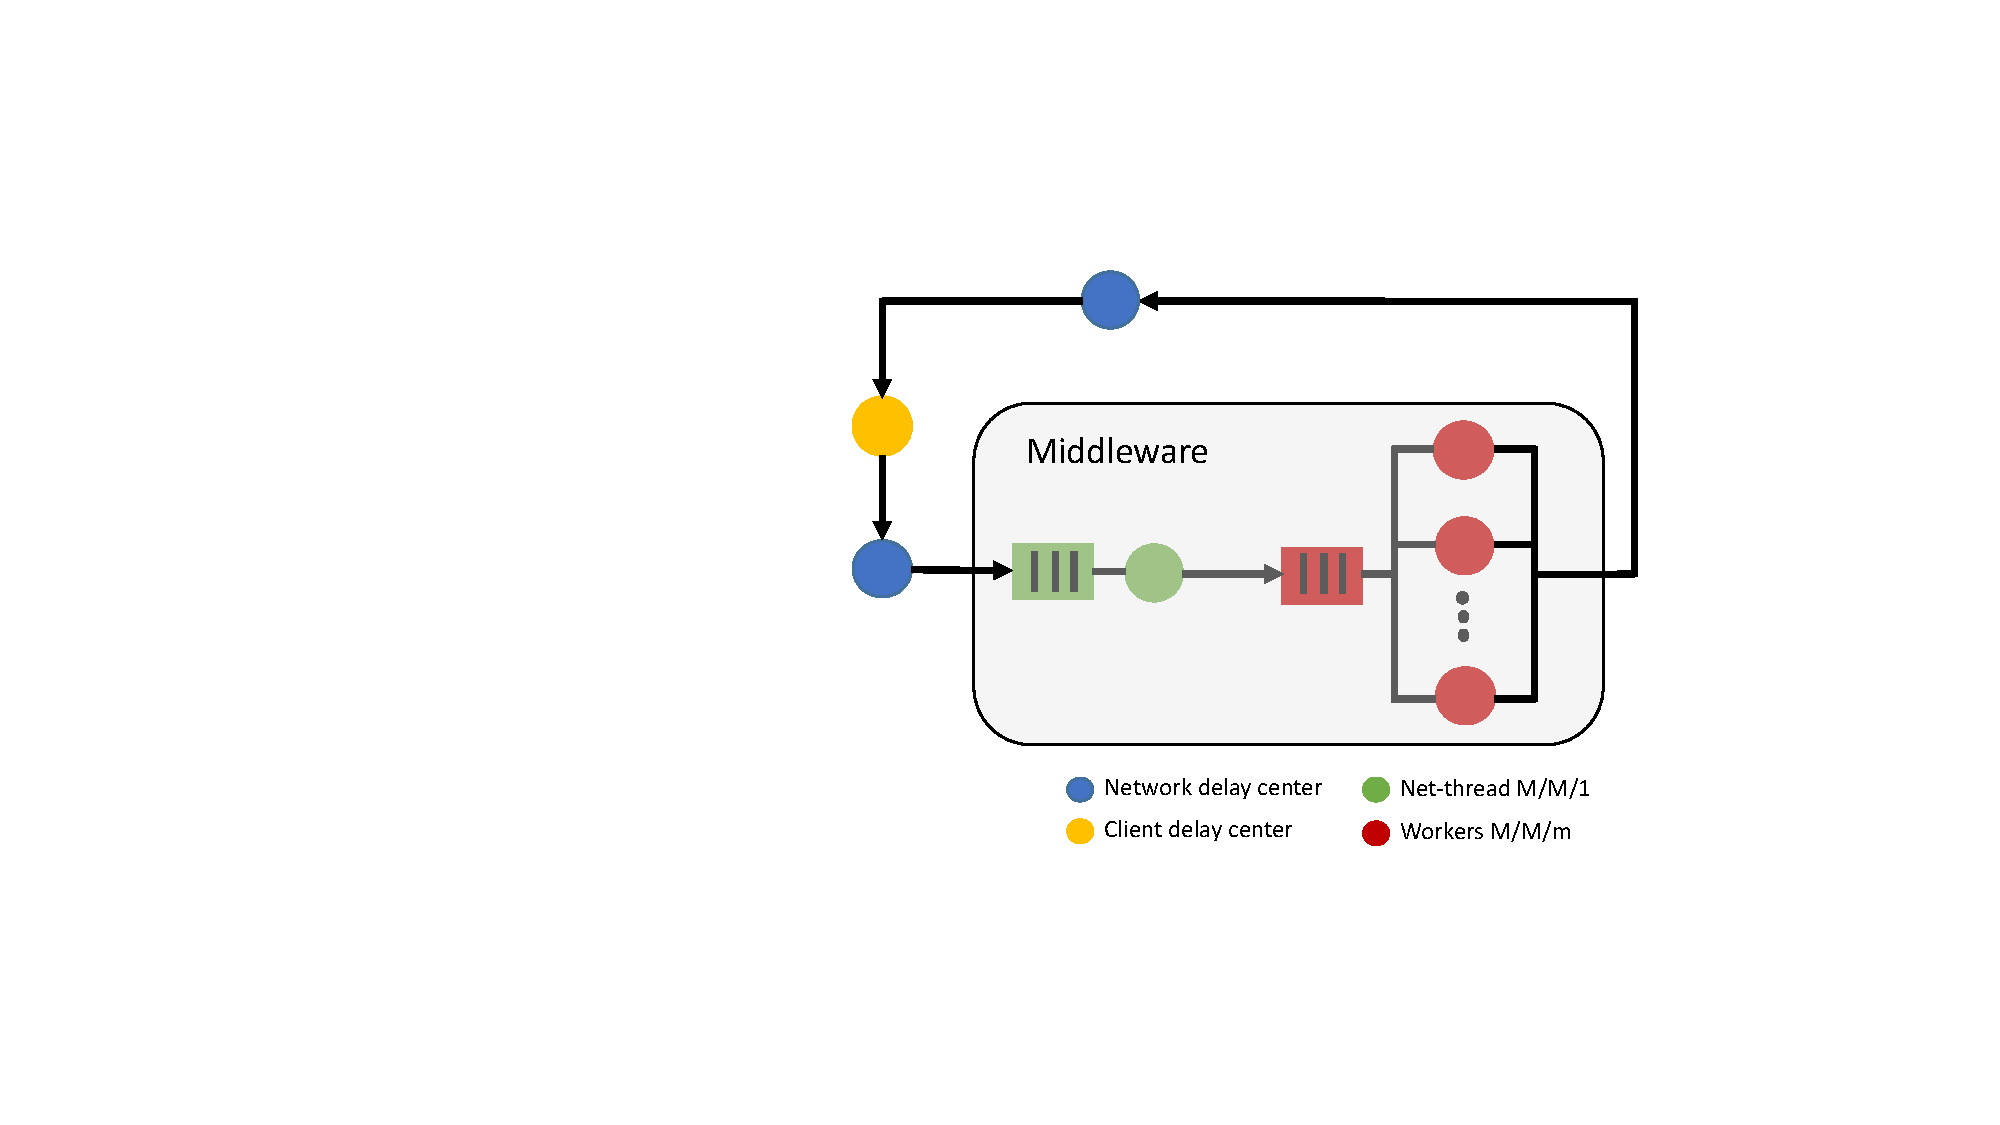
\includegraphics[scale=0.6]{figures/6_NoQ/NoQ_figure_one_mw.pdf}
	\caption{Network of queues model for one middleware.}
	\label{NoQ_one_mw}
\end{figure}

%% Input parameters of model
The \textbf{input parameters} of the model are: \\
- worker service time and number of workers \\
- net-thread service time \\
- delays of the delay centers \\
- number of jobs circulating (= number of clients) \\
- visit ratios \\

%% Present and explain the predictions
Predicted metrics (from the output of Octave) and measured metrics for 8 workers and 48 client-load are shown in Table \ref{table:noq_1midd}. 
The predictions for the system throughput and the response time of the middleware are quite accurate. The predictions for the length of the internal request queue are slightly overestimated. This is because $Q_{workers}$ actually not only includes the jobs waiting in the queue but also those receiving service at the workers. Note that there can be at most 8 jobs receiving service at the workers at the same time since we have 8 workers. \\
In contrast to the previous models, a network of queues allows us to do a bottleneck analysis. For the read-only workload, the bottleneck in our system of Section \ref{sec:baselineWithMWOne} was the memcached server respectively its outbound network bandwidth. This is correctly predicted by the model since $U_{workers} > U_{netthread}$ and based on our model $U_{workers}$ includes the memcached server. For the write-only workload, the bottleneck in our system (for 8 worker threads) were the worker threads, which is also correctly predicted as $U_{workers} > U_{netthread}$. The bottlenecks are at $100\%$ utilization which conforms to our system which is also saturated at 48 client-load with 8 worker threads for both read-only and write-only workloads.

If we compare read-only and write-only net-thread utilization, we see that the net-thread utilization for write-only is 5x higher than for read-only. This is because the Set requests are bigger and thus the net-thread needs to read more data in contrast to the Get requests which just contain a key. 

Another interesting point to mention is that if we do the write-only workload analysis for 64 workers, we have $58.11\%$ utilization for the net-thread and $26.65\%$ for the workers. Thus the model predicts that the bottleneck is on the net-thread and not on the worker threads anymore which exactly corresponds to the bottleneck analysis done in Section \ref{sec:baselineWithMWOne} as for higher number of workers the worker bottleneck is removed.

\begin{table}[!ht]
	\begin{adjustbox}{center}
		\begin{tabulary}{\linewidth}{ C | C | C | C | C | }
			\cline{2-5}	&	\multicolumn{2}{| c |}{\textbf{read-only}}	&	\multicolumn{2}{| c |}{\textbf{write-only}}	\\
			\cline{2-5} &	predicted	&	measured	&	predicted	&	measured	\\
			\hline	\multicolumn{1}{| c |}{throughput $X$ [req/s]}		&	2'964.4	&	2'938.08	&	7'255.6	&	7'112.42	\\
			\hline	\multicolumn{1}{| c |}{response time $R_{mw}$ [ms]}		&	15.26	&	15.4	&	5.59	&	5.74	\\
			\hline	\multicolumn{1}{| c |}{queue length $Q_{workers}$}				&	45.16	&	34.31	&	40.17	&	32.51	\\
			\hline	\multicolumn{1}{| c |}{utilization $U_{netthread}$ [\%]}	&	6.28	&	-		&	30.02	&	-	\\
			\hline	\multicolumn{1}{| c |}{utilization $U_{workers}$ [\%]}	&	100	&	-		&	100	&	-	\\
			\hline 
		\end{tabulary}
	\end{adjustbox}	
	\caption{\textit{Network of Queues for 8 workers and 48 client-load (one middleware)}.}
	\label{table:noq_1midd}
\end{table}

\subsubsection{System with two middlewares}
%% Explain model
The model is shown in Figure \ref{NoQ_two_mws}. 
Essentially everything is the same as in the one middleware case, but now the middleware part is duplicated i.e. the net-thread component is duplicated and also the worker thread component is duplicated. The traffic is split equally at the client among both net-threads.

\begin{figure}[!ht]
    \centering
	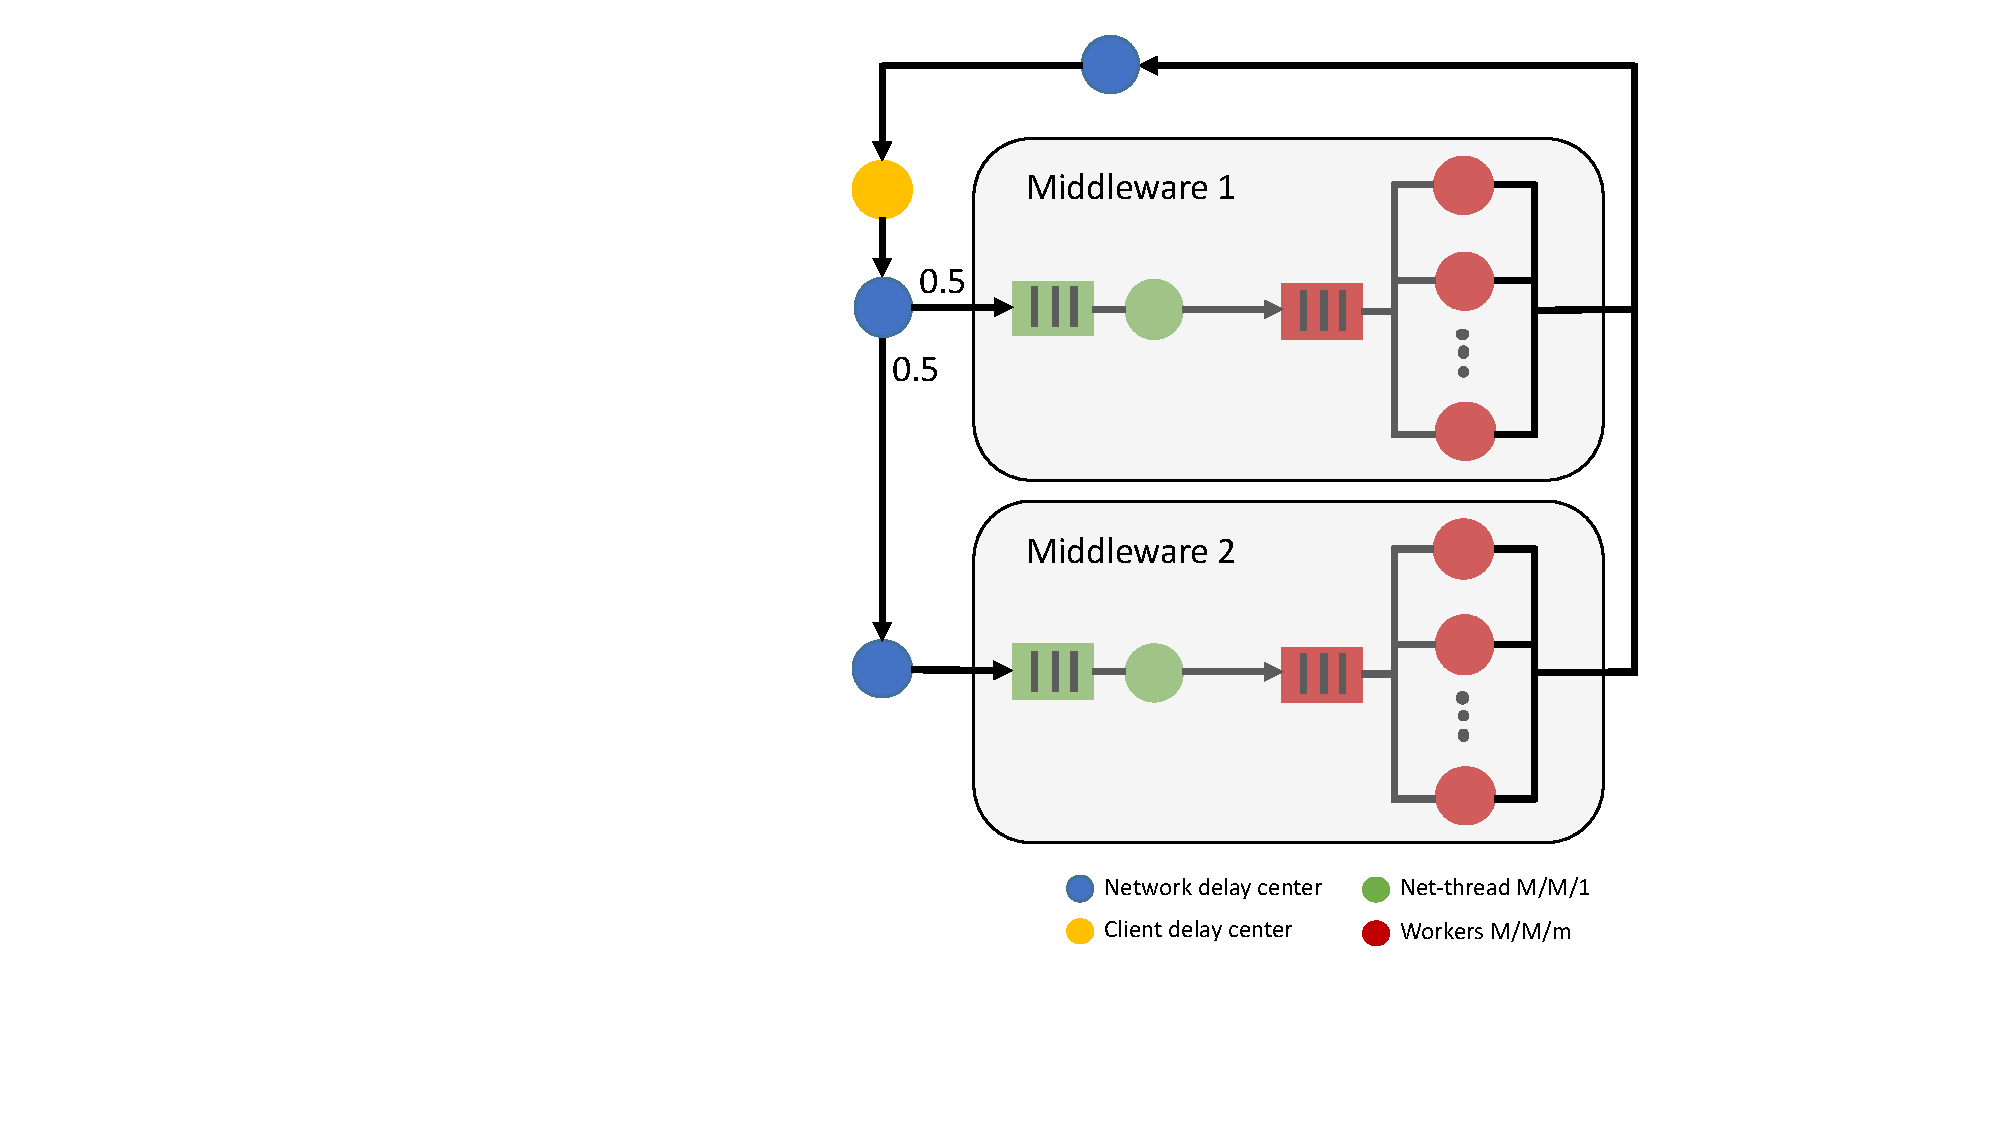
\includegraphics[scale=0.6]{figures/6_NoQ/NoQ_figure_two_mws.pdf}
	\caption{Network of queues model for two middlewares.}
	\label{NoQ_two_mws}
\end{figure}

%% Present and explain the predictions
Predicted metrics (from the output of Octave) and measured metrics for 8 workers and 48 client-load are shown in Table \ref{table:noq_2midd}. 
Again the model predicts the throughput and response time of the middlewares quite accurately. The queue length is slightly overestimated for the same reason that was given in the one middleware case. \\
For the read-only workload the predicted bottleneck are the worker threads because $U_{workers} > U_{netthread}$. This conforms to our bottleneck analysis in Section \ref{sec:baselineWithMWTwo} where the memcached server is the bottleneck, because again the servers are part of the M/M/m component representing the worker threads. 
For the write-only workload, the predicted bottleneck are also the worker threads for the same reason, which conforms to our bottleneck analysis in Section \ref{sec:baselineWithMWTwo} where the worker threads are the bottleneck. The bottlenecks are almost at $100\%$ utilization, which conforms to our system which is also saturated at 48 client-load with 8 worker threads for both read-only and write-only workloads.\\

If we compare the one middleware model predictions with the two middlewares model predictions, we see that especially for the write-only workload the utilization of the net-thread is significantly reduced going from one to two middlewares. 
This is because the two net-threads share the same load and we have less congestion in front of the Java Selector objects for the two middlewares configuration. 
\begin{table}[!ht]
	\begin{adjustbox}{center}
		\begin{tabulary}{\linewidth}{ C | C | C | C | C | }
			\cline{2-5}	&	\multicolumn{2}{| c |}{\textbf{read-only}}	&	\multicolumn{2}{| c |}{\textbf{write-only}}	\\
			\cline{2-5} &	predicted	&	measured	&	predicted	&	measured	\\
			\hline	\multicolumn{1}{| c |}{throughput $X$ [req/s]}		&	2'869.2	&	2'944.13	&	9'184.1	&	9'406.65	\\
			\hline	\multicolumn{1}{| c |}{response time $R_{mw}$ [ms]}		&	15.66	&	15.32	&	4.27	&	4.21	\\
			\hline	\multicolumn{1}{| c |}{queue length $Q_{workers}$}				&	22.44	&	11.63	&	19.47	&	10.67	\\
			\hline	\multicolumn{1}{| c |}{utilization $U_{netthread}$ [\%]}	&	2.06	&	-		&	13.98	&	-	\\
			\hline	\multicolumn{1}{| c |}{utilization $U_{workers}$ [\%]}	&	97.24	&	-		&	96.68	&	-	\\
			\hline 
		\end{tabulary}
	\end{adjustbox}	
	\caption{\textit{Network of Queues for 8 workers and 48 client-load (two middlewares)}.}
	\label{table:noq_2midd}
\end{table}

%% Conclusion
To conclude, we can say that the network of queues model provides accurate predictions of our system. But also network of queues have their limitations, and for example do not allow us to model the memcached servers and workers separately from each other. 